\section{On-chain Protocol}\label{sec:on-chain}

We describe the details of the \emph{on-chain} protocol controlling a
Hydra head (see Fig.~\ref{fig:SM_states_basic}) using the CEM abstraction \&
notation (see Section~\ref{sec:cem}). In addition of standard CEM modeling, we
also provide the formal conditions $\cemTxCon$ which a transition need to
satisfy and also include them in the accompanying text.

The following sections describe the structure of each of the transactions
comprising the Head protocol: $\mtxInit{}$, $\mtxCom{}$, $\mtxAbort{}$,
$\mtxCollect{}$, $\mtxClose{}$, $\mtxContest{}$, and $\mtxFanout{}$. Following
the EUTxO model, this structure is enforced on-chain through \emph{validators}
which are \emph{scripts instances} attached to each UTxO and run as part of the
ledger's validation of the transaction (see Section~\ref{sec:eutxo}). The
protocol defines one minting policy script and three validator scripts:
\begin{itemize}
  \item $\muHead$ governs the minting of state and participation tokens,
  \item $\nuInitial$ controls initialization and how UTxOs are committed to the head, while
  \item $\nuCommit$ controls the collection of committed UTxOs into the head, and lastly
  \item $\nuHead$ controls the main protocol state-machine logic.
\end{itemize}

\subsection{Init transaction}

The \mtxInit{} transaction creates a head instance and establishes the initial
state of the protocol and is shown in Figure~\ref{fig:SM_commit_tx}. The head
instance is represented by the unique\footnote{As the EUTxO ledger preventing
  double-spending, the uniqueness of $\cid$ is guaranteed because $i_{seed}$ can
  only be spent once} currency identifier $\cid$ created by minting tokens using
the parameterized $\muHead$ minting policy script:
\[
  \cid = \hash(\muHead(i_{seed}))
\]
\noindent where $i_{seed} \in \txInputs$ is a transaction input and the
$\muHead(i_{seed})$ minting policy validator checks:
\begin{menumerate}
  \item $i_{seed}$ is spent in this transaction
  $i_{seed} \in \txInputs$
\end{menumerate}

\vspace{0.1cm}
\noindent Two kinds of tokens are minted:
\begin{itemize}
  \item A single \emph{State Thread (ST)} token marking the output carrying the state
        of the protocol on-chain, whose name is the well known string
        \texttt{HydraHeadV1}, i.e.
        $\st = (\cid \rightarrow \texttt{HydraHeadV1} \rightarrow 1)$
  \item One \emph{Participation Token (PT)} per participant
        $i \in \{1 \dots \nop \}$, where the token name is the participant's
        verification key hash $k_i^{\#}$, i.e.
        $\pt_{i} = (\cid \rightarrow k_{i}^{\#} \rightarrow 1)$.
\end{itemize}

\noindent Consequently, the \mtxInit{} transaction

\begin{itemize}
  \item has at least input $i_{seed}$,
  \item mints one $\st$ and one $\pt$ for each of the $\nop$ participants with
        policy $\cid :: \{\st, \pt_{1}, \ldots, \pt_{\nop}\}$,
  \item has one state-machine output locked by $\nuHead$ with datum
        $\datum_{\mathsf{head}}$
  \item has $\nop$ outputs, where each output is locked by $\nuInitial$ and the
        $\ith i$ output has the participation token $\pt_i$ in its value, and
        $\mathsf{cid}$ as datum.
\end{itemize}

\noindent The initial state of the protocol is captured in the state-machine output datum
\[
  \datum_{\mathsf{head}} = (\stInitial,\cid,\hpAK,\hppuv,\nop,\cPer)
\]
where
\begin{mitemize}
  \item $\stInitial$ is a state identifier,
  \item $\cid$ is the unique currency id of this instance,
  \item $\hpAK$ is the aggregated off-chain multi-signature key established during the
  setup phase,
  \item $\hppuv$ is the list of all participants verification keys
  $(k_1,\ldots,k_\nop)$ exchanged during the setup phase and identifying the
  head members on-chain,
  \item $\nop$ is the number of head participants, and
  \item $\cPer$ is the length of the contestation period.
\end{mitemize}

\noindent Validator $\nuInitial$ ensures that the output is consumed by either
an \mtxAbort{} (see Section~\ref{sec:abort-tx} below) or a \mtxCom{} (see
Section~\ref{sec:commit-tx} below) transaction. Note that the general
well-formedness and validity of the \mtxInit{} transaction is checked on the
mainchain, but head members need to additionally check whether the initial state
has the right $\cid$ and is consistent with parameters agreed during setup.

\begin{figure}[h]

  \centering

  % 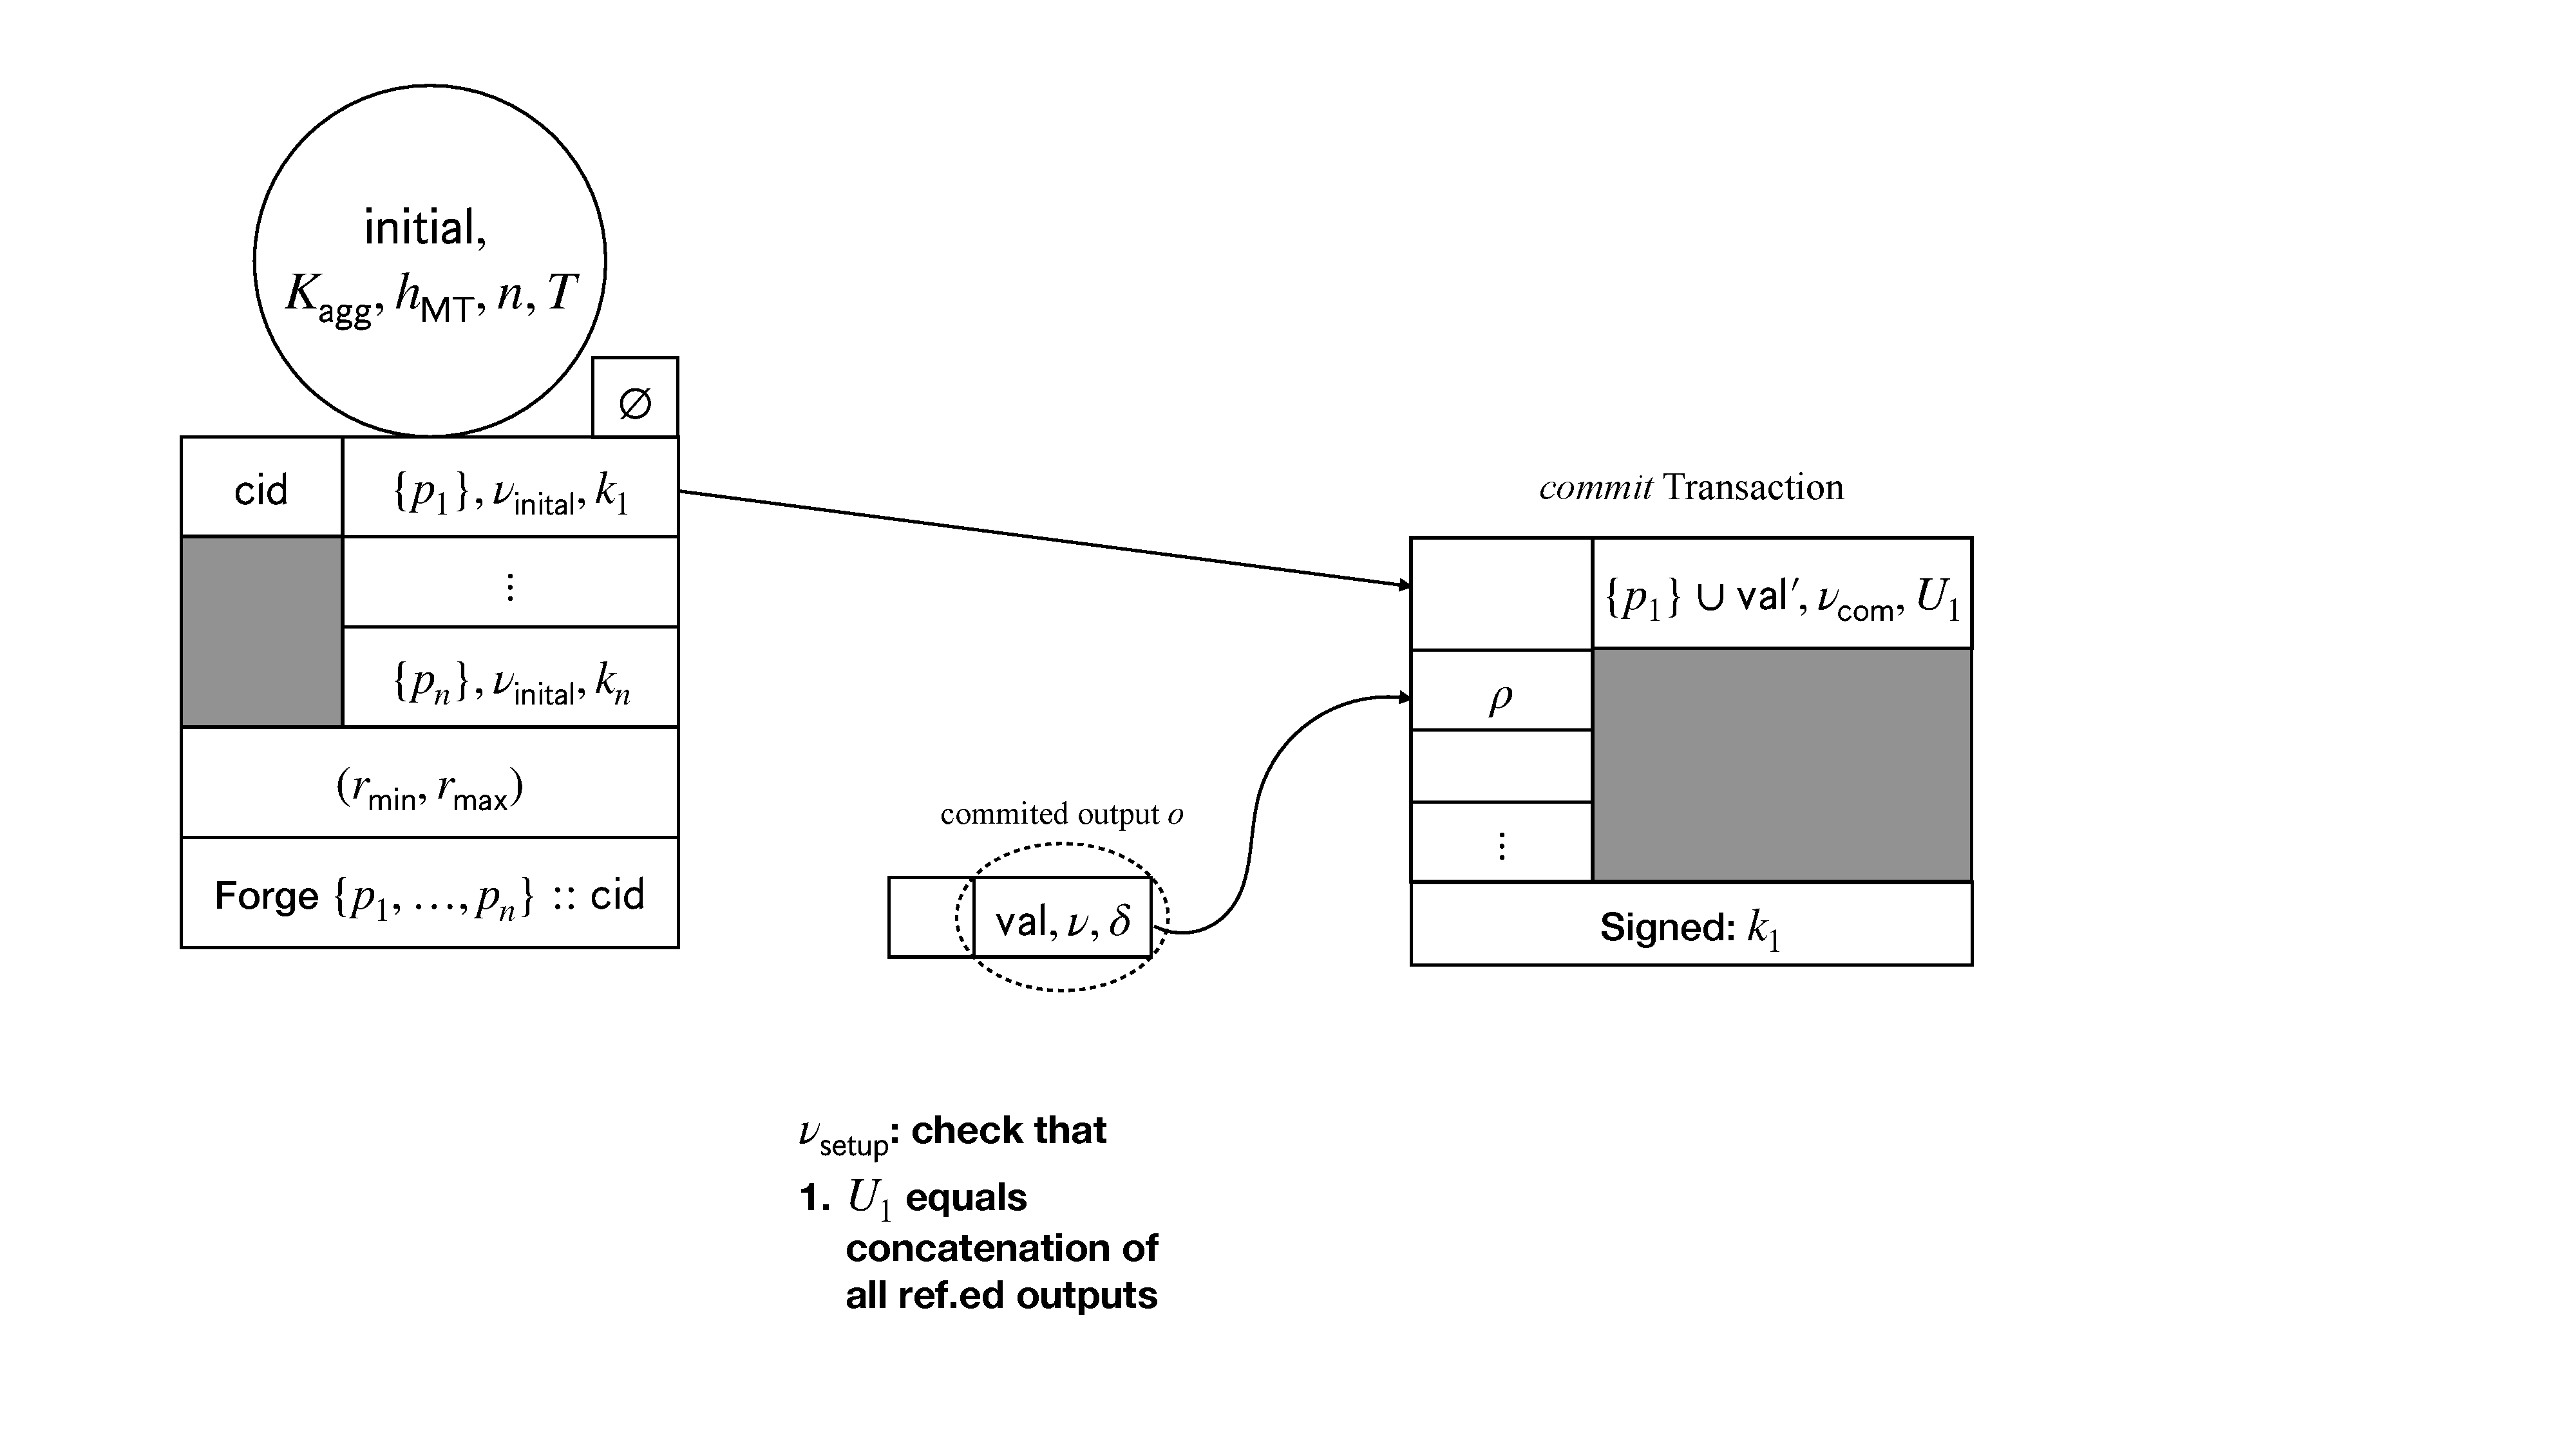
\includegraphics[width=\textwidth/2,trim=130 330 430 50,clip]{figures/SM_commit_tx.pdf}

  % TODO: clean draw marked up version
  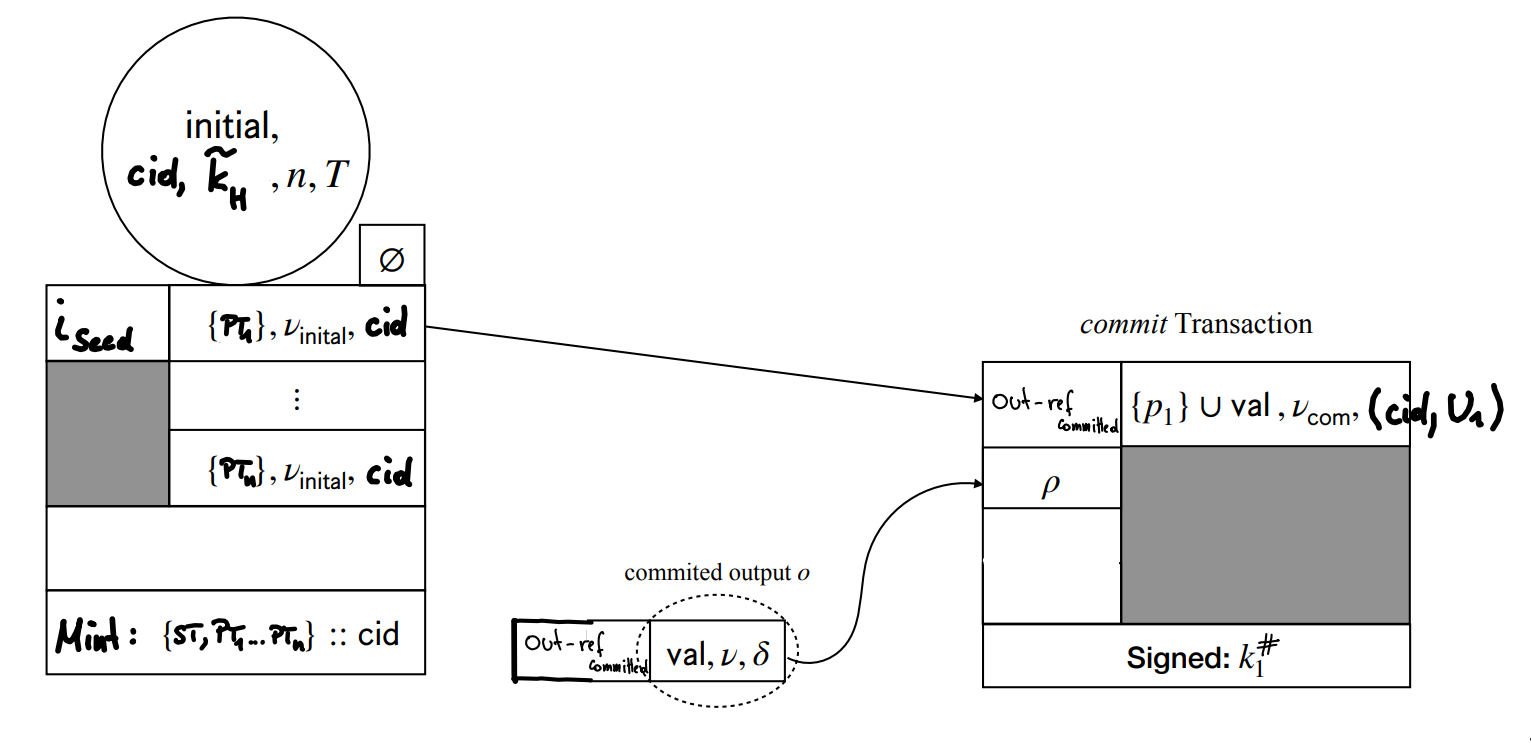
\includegraphics[width=\textwidth*2/3]{figures/SM_commit_tx.png}

  \caption{
    \mtxInit{} transaction (left) with one \mtxCom{} transaction
    (right) attached locking one output (center).}\label{fig:SM_commit_tx}

\end{figure}


%%% Local Variables:
%%% mode: latex
%%% TeX-master: "main"
%%% End:


\subsection{Commit Transaction}\label{sec:commit-tx}

A \mtxCom{} transaction is depicted in Figure~\ref{fig:SM_commit_tx} and has the following structure:
\begin{itemize}
    \item One input $i_{\mathsf{initial}} = (\txOutRef_{initial}, \rho_{initial})$ consuming $o_{initial} = (\val_{initial}, \nuInitial, \delta_{initial})$,
    \item Zero or one input with reference $\txOutRef_{commit}$ consuming output $o_{commit} = (.,\val_{commit},.)$,
    \item One output $o_{com} =  (\val_{com}, \nuCommit, \delta_{com}).$
\end{itemize}

\noindent The $\nuInitial$ validator ensures the transaction has the following structure:
\begin{menumerate}
    \item Transaction is signed by correct participant: $\txKeys = \{\mathsf{k}\}$ s.t.
    $
    \exists (\mathsf{cid} \rightarrow \mathsf{PT}_i \rightarrow 1) \in \val_{com}, \hash(\mathsf{k}) = \mathsf{PT}_i,
    $ \todo{check against PT or against datum ($\hppuv$)? or both?}
    \item The initial redeemer references the committed output, $\rho_{initial} = \txOutRef_{commit}$,
    \item The initial datum is $\mathsf{cid}$,
    \item The committed value is in the output $\val_{com} = \{(\mathsf{cid} \rightarrow \mathsf{PT}_i \rightarrow 1)\} \cup \val_{commit} $,
    \item The committed output is serialised as the datum of $o_{com}$: $\delta_{com} = (\mathsf{cid}, U)$, with \\ $U = (\txOutRef_{commit},\bits(o_{commit}))$
    \item No minting or burning happens.
\end{menumerate}

\noindent The $\nuCommit$ validator ensures the output is collected by either a \mtxCCom{} or \mtxAbort{} transaction of the on-chain state machine.

\subsection{CollectCom Transaction}

\begin{figure}[h]

  \centering

  % 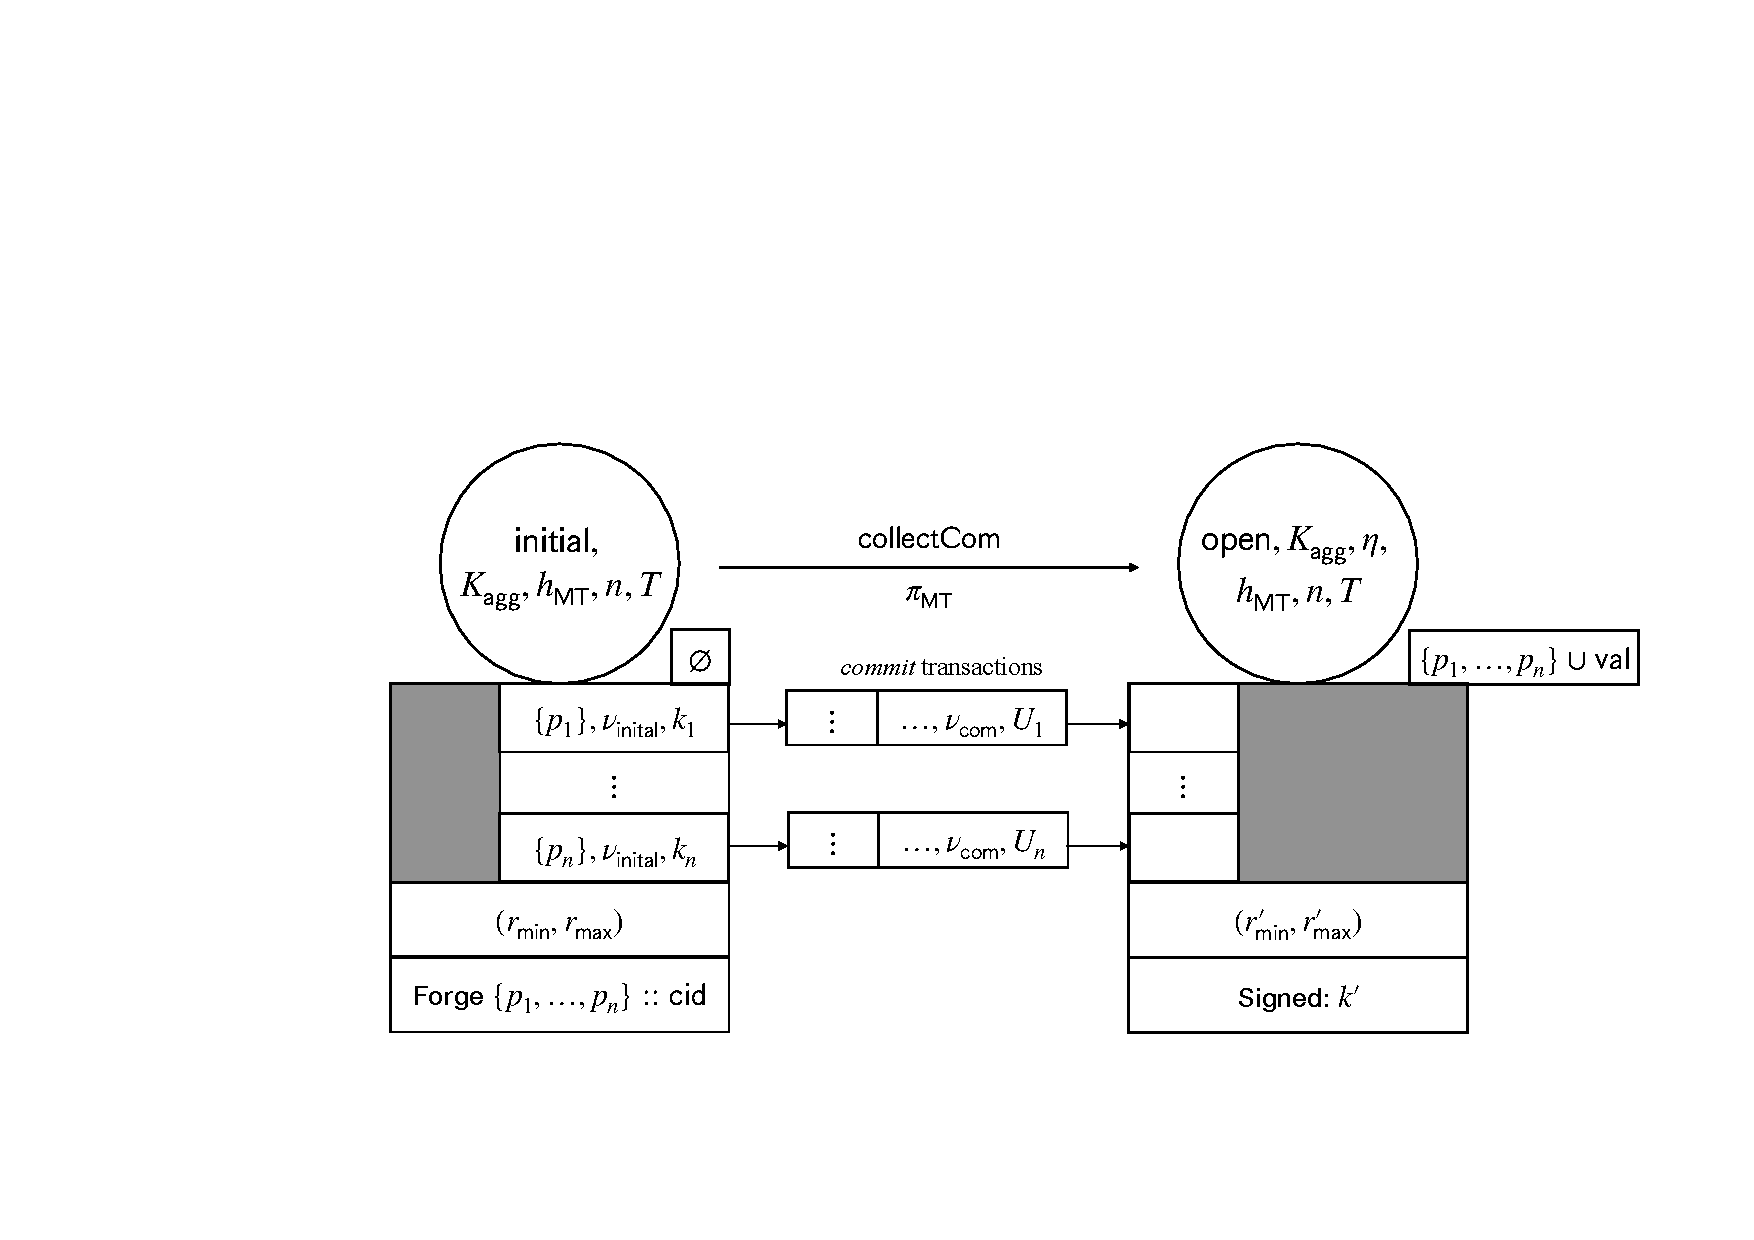
\includegraphics[width=\textwidth/2]{figures/SM_initial_open.pdf}
  %
  % TODO: clean draw marked up version
  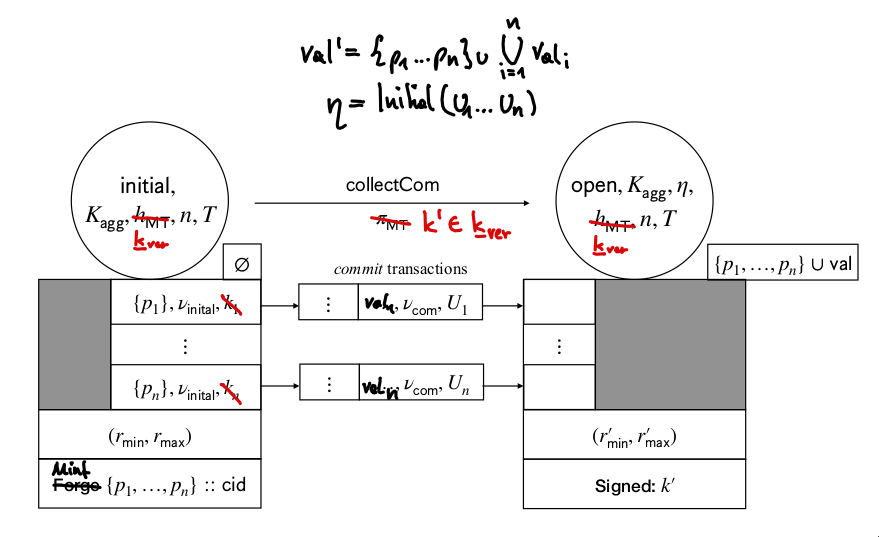
\includegraphics[width=\textwidth/2]{figures/SM_initial_open.png}

  \caption{\mtxInit{} transaction (left) with \mtxCCom{} transaction
    (right) and \mtxCom{} transactions (center).}
  \label{fig:SM_initial_open}

\end{figure}



%%% Local Variables:
%%% mode: latex
%%% TeX-master: "main"
%%% End:


The \mtxCCom{} transaction collects all outputs from \mtxCom{} transactions participating in the same head and advances the state of the CEM state machine:
$$
   (\stInitial,\hpAK,\hppuv,\nop,\cPer) \xrightarrow{\mathsf{collectCom}} (\stOpen,\hpAK,\eta,\hppuv,\nop,\cPer),
$$
where $\eta$ is the hash of the concatenation of the serialised representation of committed outputs:
$$
\eta = \hash(\bigoplus_{i=1}^n \bytes(U_i)).
$$

\noindent The $\nuHead$ validator additionally checks that:
\begin{menumerate}
  \item All committed value captured and no additional funds ``enter'' or ``leave''
  $\val' = \{\mathsf{ST}\} \cup \bigcup_{i=1}^{n} \mathsf{PT}_{i} \cup \val_{i}$,
  \item All tokens present in output
  $|\{cid \rightarrow . \rightarrow 1\} ~ \mathsf{in} ~ \val'| = \nop + 1$,
  \item Signer is one of the participants: $\txKeys = \{\mathsf{k'}\}$, $k' \in \hppuv$ and
    $
    \exists (\mathsf{cid} \rightarrow \mathsf{PT}_i \rightarrow 1) \in \val, \hash(\mathsf{k'}) = \mathsf{PT}_i,
    $
  \item Unchanged parameters $\mathsf{cid}$, $\hpAK$, $\hppuv$, $\nop$, and
  $\cPer$ in the data field,
  \item No minting or burning happens.
\end{menumerate}

\noindent Each of the $\nuCommit^i$ validators, for $i \in \{ 1\dots n\}$, additionally checks:
\begin{menumerate}
    \item The ST token is present in the output value $(cid \rightarrow ST \rightarrow 1) \in \val'$, where $(cid,.) = \delta_{com}$ is given by the datum of the commit output $o_{com}$.
\end{menumerate}

\subsection{Abort Transaction}\label{sec:abort-tx} 

\begin{figure}

  \centering

  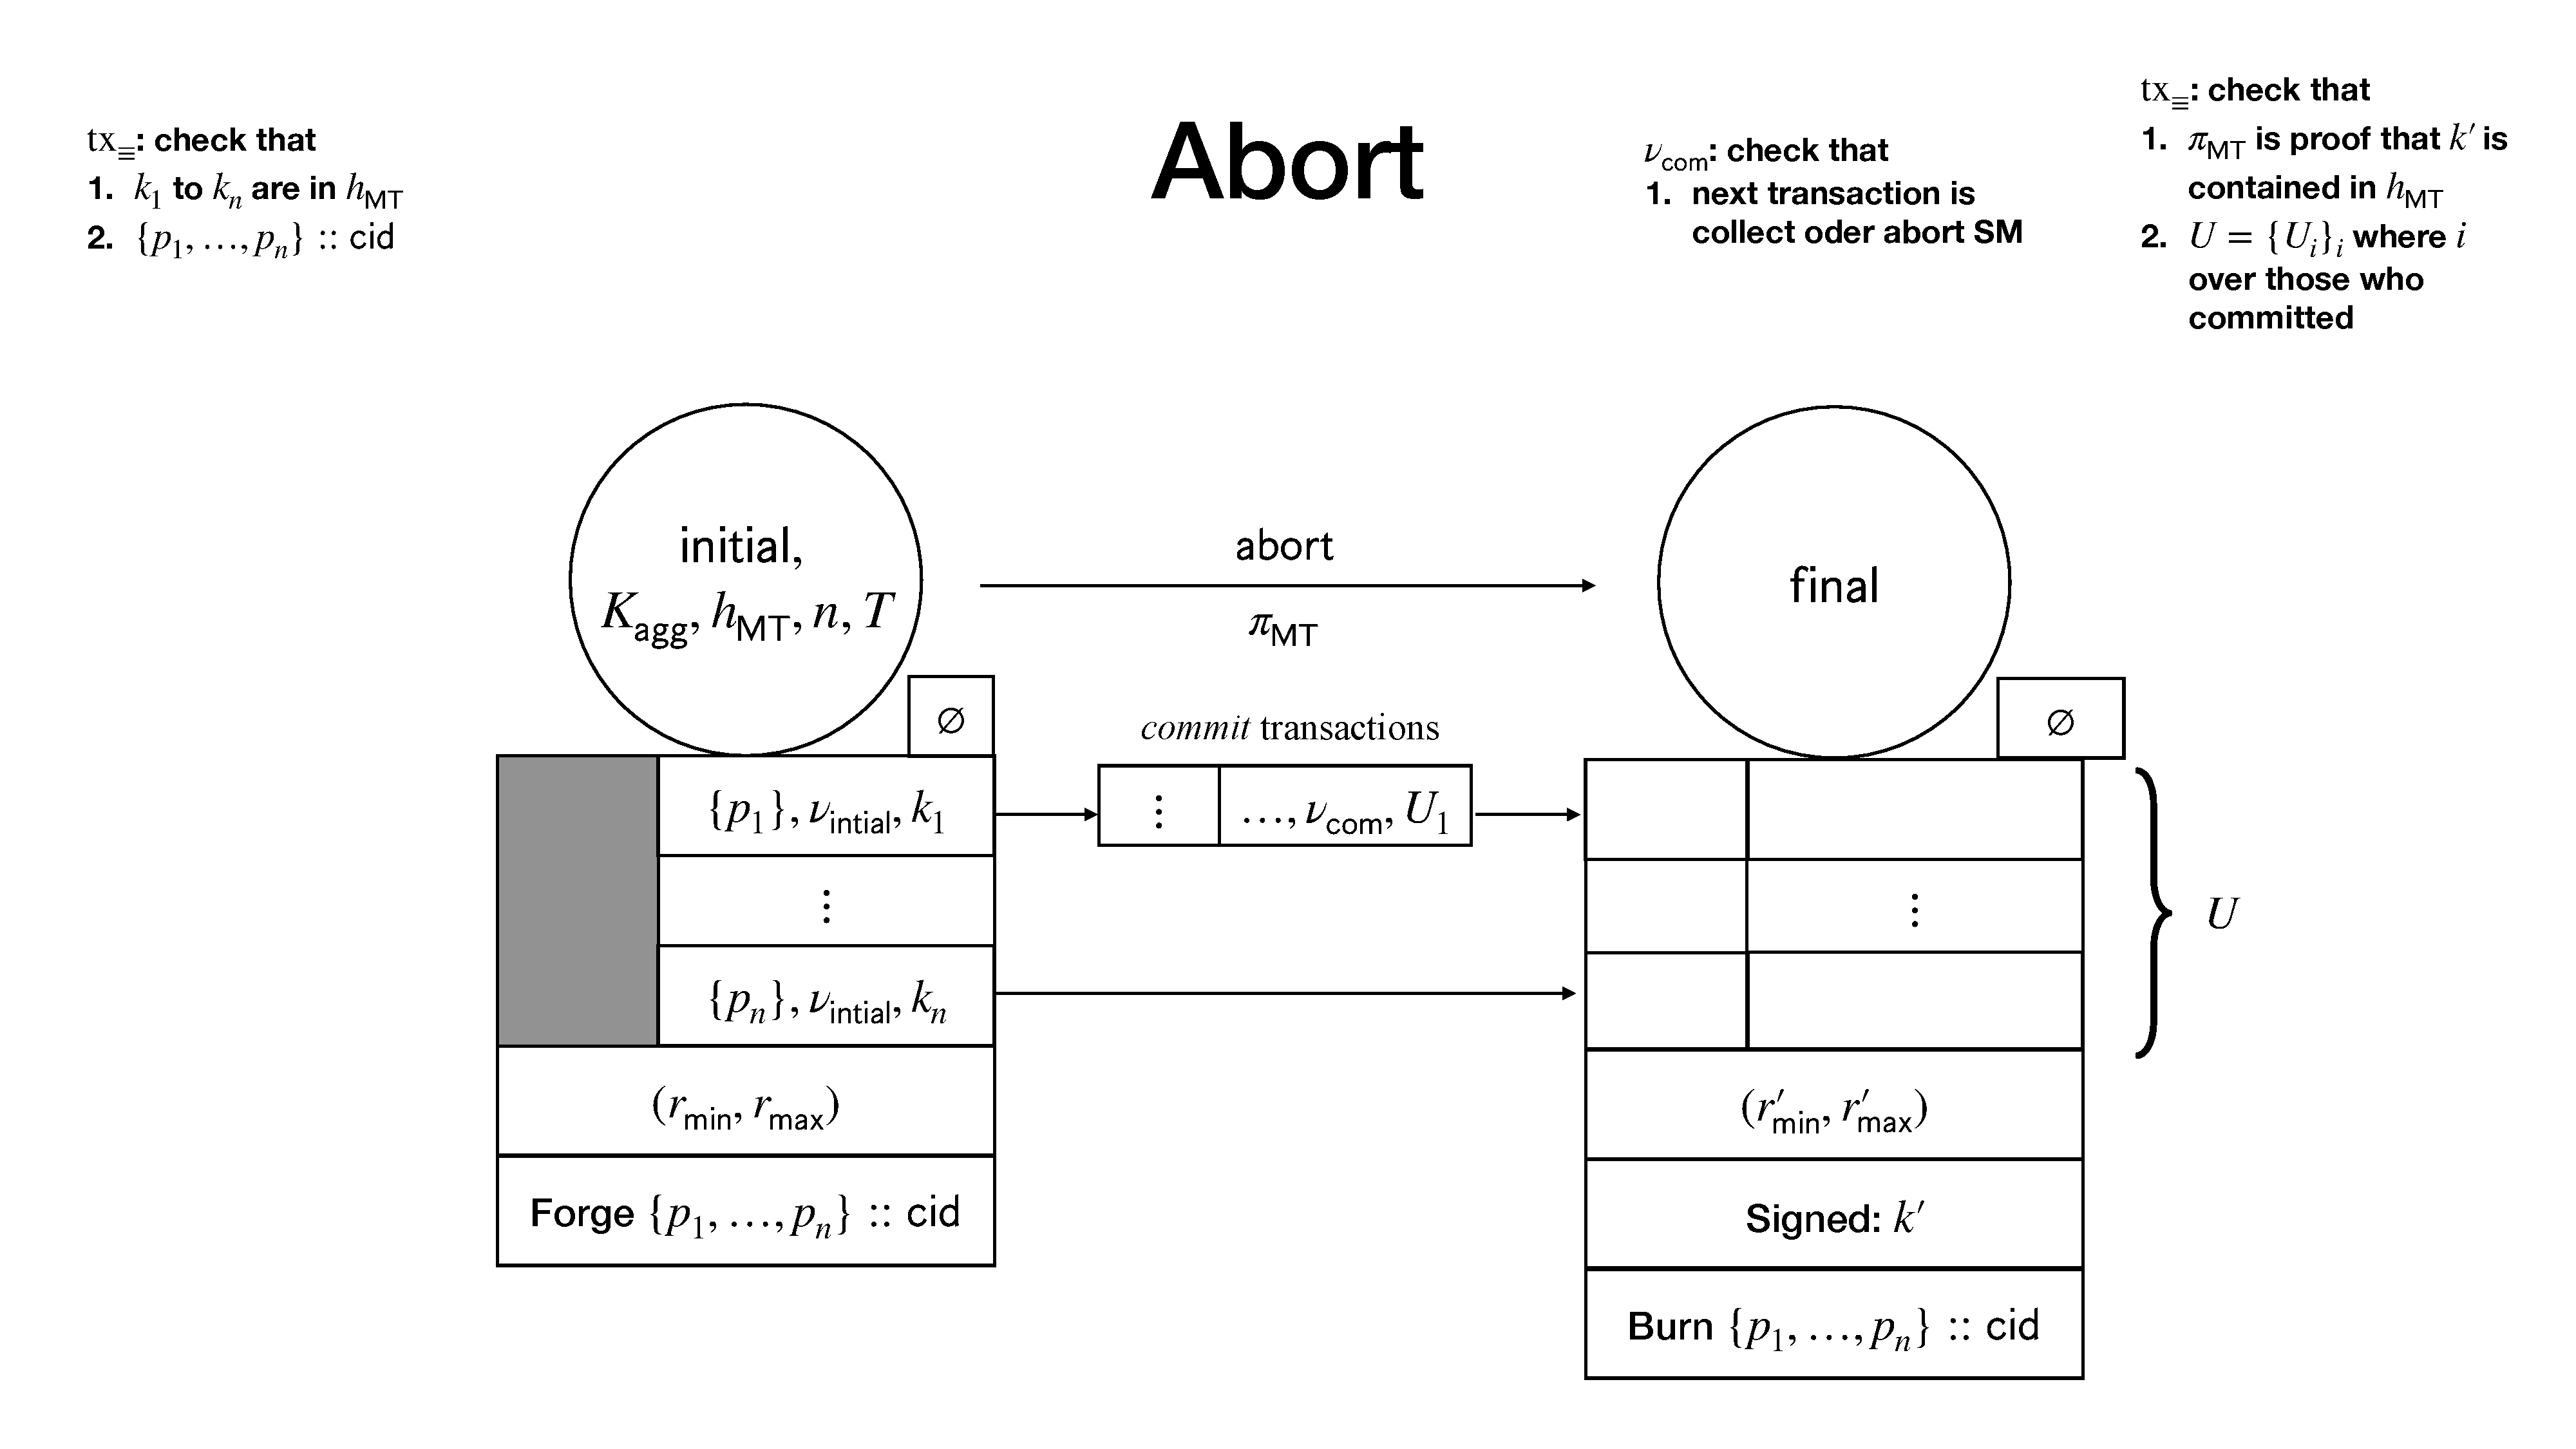
\includegraphics[width=\textwidth/2-2em,trim=350 20 240 300,
  clip]{figures/SM_initial_final.pdf}
    
  \caption{\mtxInit{} transaction (left) with \mtxAbort{} transaction
    (right) and \mtxCom{} transactions (center).}
  \label{fig:SM_initial_final}

\end{figure}



%%% Local Variables:
%%% mode: latex
%%% TeX-master: "main"
%%% End:



The \mtxAbort{} transaction
(see Fig.~\ref{fig:SM_initial_final}) allows a party to abort the
creation of a head.  The state is transitioned to $\mathsf{final}$:

$$
   (\stInitial,\hpAK,\hppuv,\nop,\cPer) \xrightarrow{\mathsf{abort}} \stFinal.
$$

\noindent The $\nuHead$ validator ensures that:
\begin{menumerate}
 \item All outputs committed into the head are recreated as is: $\forall i \in \{1\dots\nop\}, \hash(O_\sigma[i]) = \delta_i$,
  \item Signer is one of the participants: $\txKeys = \{\mathsf{k'}\}$, $k' \in \hppuv$ and
    $
    \exists (\mathsf{cid} \rightarrow \mathsf{PT}_i \rightarrow 1) \in \val, \hash(\mathsf{k'}) = \mathsf{PT}_i,
    $
 \item All participation tokens are burnt: $\forall i \in \{1\dots\nop\}, \{\mathsf{cid} \rightarrow \mathsf{PT}_i \rightarrow -1\} \subseteq \mathsf{Mint}.$\todo{number of tokens burned vs. explicit enumeration what to burn?}
\end{menumerate} 

\noindent For each of the $\nuInitial$ validators consumed, checks:
\begin{menumerate}
  \item The ST is getting burned
  $\{cid \rightarrow "HeadV1" \rightarrow -1\} \subseteq \mathsf{Mint}$, where
  $cid = \delta_{initial}$ is given by the datum of the spent initial output.
\end{menumerate}

\noindent For each of the $\nuCommit$ validators consumed, checks:
\begin{menumerate}
  \item The ST token is getting burned
  $\{cid \rightarrow ST \rightarrow -1\} \subseteq \mathsf{Mint}$, where
  $(cid,.) = \delta_{com}$ is given by the datum of the spent commit output.
\end{menumerate}

\subsection{Close Transaction}\label{sec:close-tx}

\begin{figure}[t!]

  \centering

  %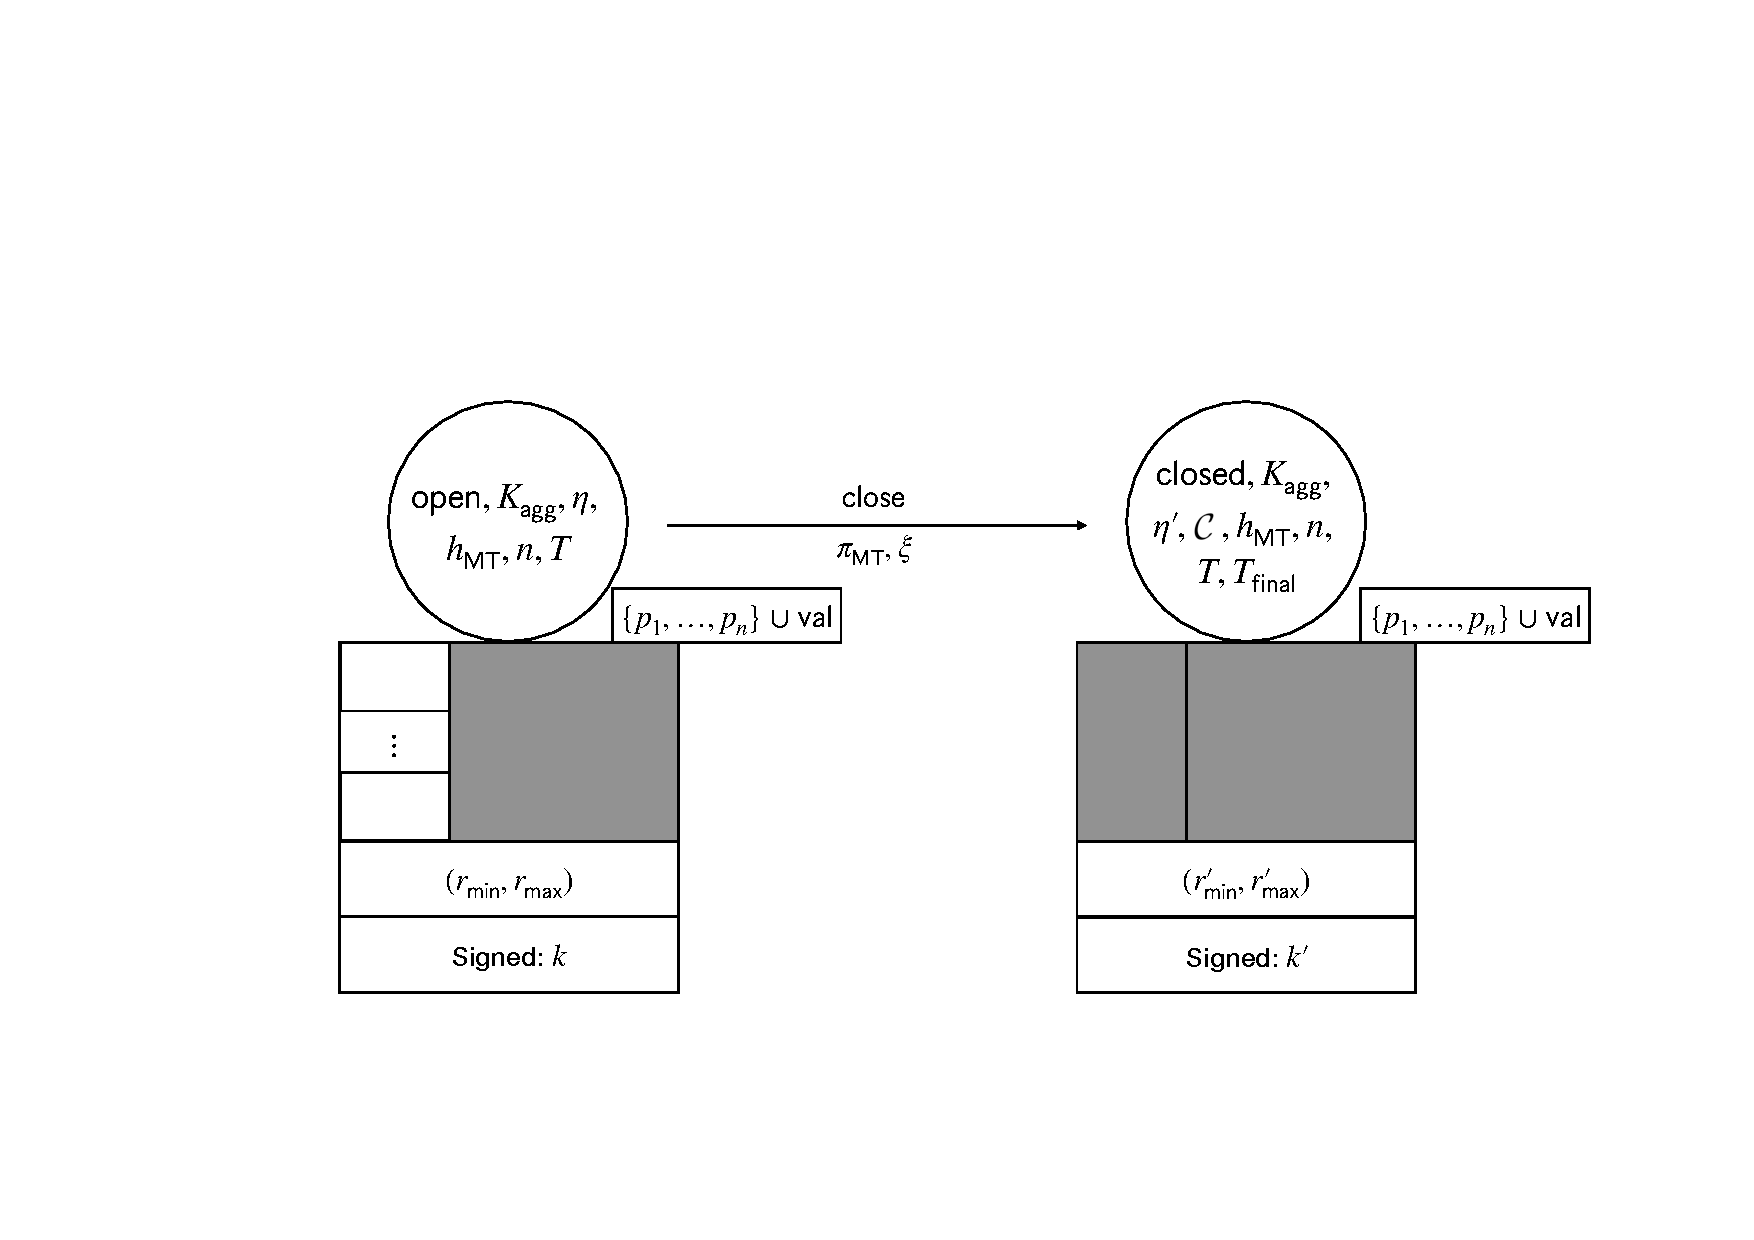
\includegraphics[width=\textwidth/2-2em,trim=350 100 160 300,
  %clip]{figures/SM_open_closed.pdf}

  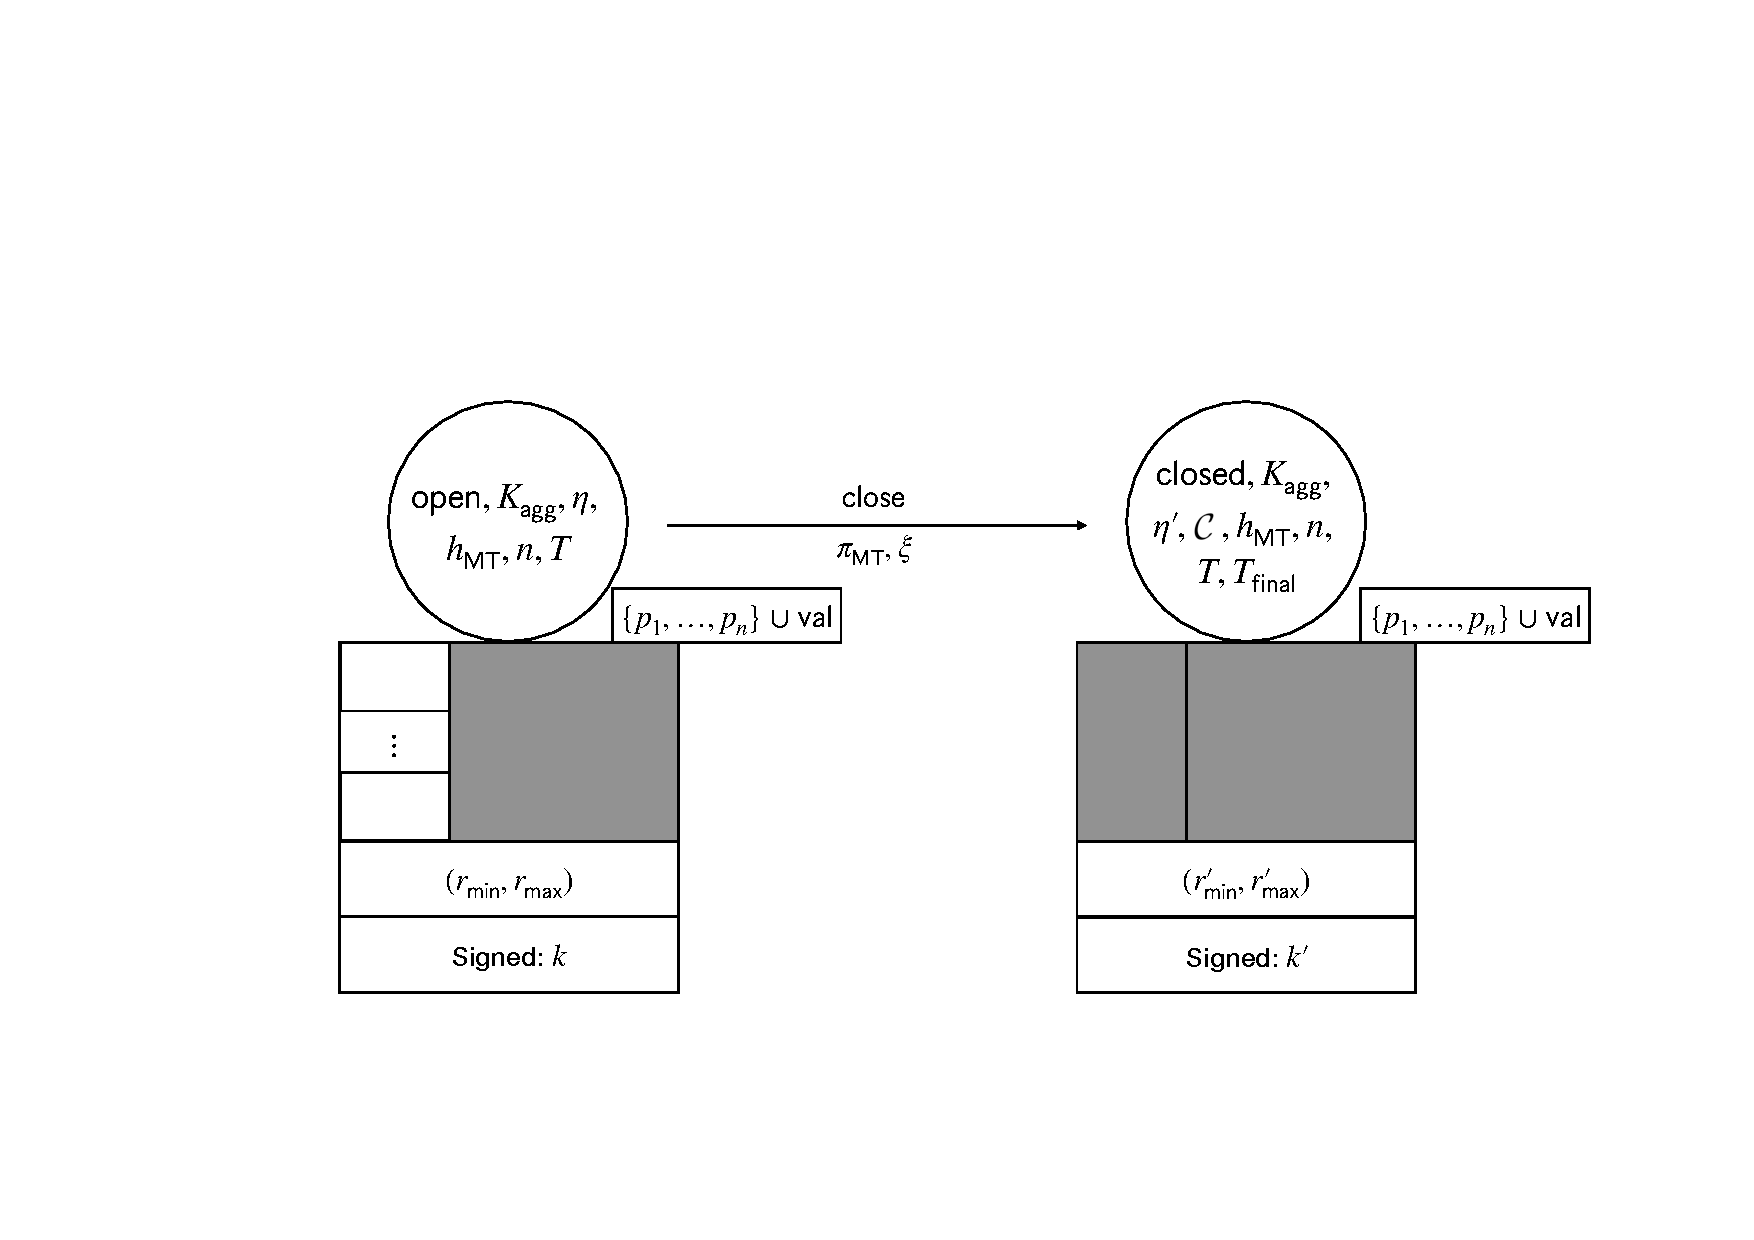
\includegraphics[width=\textwidth/2]{figures/SM_open_closed.pdf}

  \caption{\mtxCCom{} transaction (left) with \mtxClose{}
    transaction (right).}
  \label{fig:SM_open_closed}

\end{figure}



%%% Local Variables:
%%% mode: latex
%%% TeX-master: "main"
%%% End:


In order to close a head, a head member may post the \mtxClose{} transaction (see Fig.~\ref{fig:SM_open_closed}), which results in a SM transition
from the $\stOpen$ state to the $\stClosed$ state:
$$
(\stOpen,\hpAK,\eta,\hppuv,\nop,\cPer) \xrightarrow[\xi]{\mathsf{close}} (\stClosed,\hpAK,\eta',\eta_0,\mathcal{C},\hppuv,\nop,\cPer,\Tfinal) 
$$
with $\eta_0 = \eta$. \\

\noindent The $\nuHead$ validator perform those additional checks:
\begin{enumerate}
  \item Signer is one of the participants: $\txKeys = \{\mathsf{k'}\}$, $k' \in \hppuv$ and
    $
    \exists (\mathsf{cid} \rightarrow \mathsf{PT}_i \rightarrow 1) \in \val, \hash(\mathsf{k'}) = \mathsf{PT}_i,
    $
  \item $\xi$ is a valid multi-signature of $\eta'$ w.r.t. to $\hpAK$,
  \item Recorded snapshot state is consistent:
    $$
    \eta' = \left\{\begin{array}{ll}
         (s, \hash(U')), & \mathrm{if}\ s > 0,\\
         (0, \eta_0) & \mathit{otherwise} 
    \end{array}\right.,
    $$
  \item Record contestation deadline, $\Tfinal = \txRmax + T$,
  \item Ensure timeliness of the transaction $\txRmax - \txRmin \leq T$ 
  \item Initialize the set of contesters $\mathcal{C} = \emptyset$\todo{explain why in footnote}
  \item Value in the head is preserved, $val' = val$
\end{enumerate}

\subsection{Contest Transaction}\label{sec:contest-tx}

\begin{figure}

  \centering

  %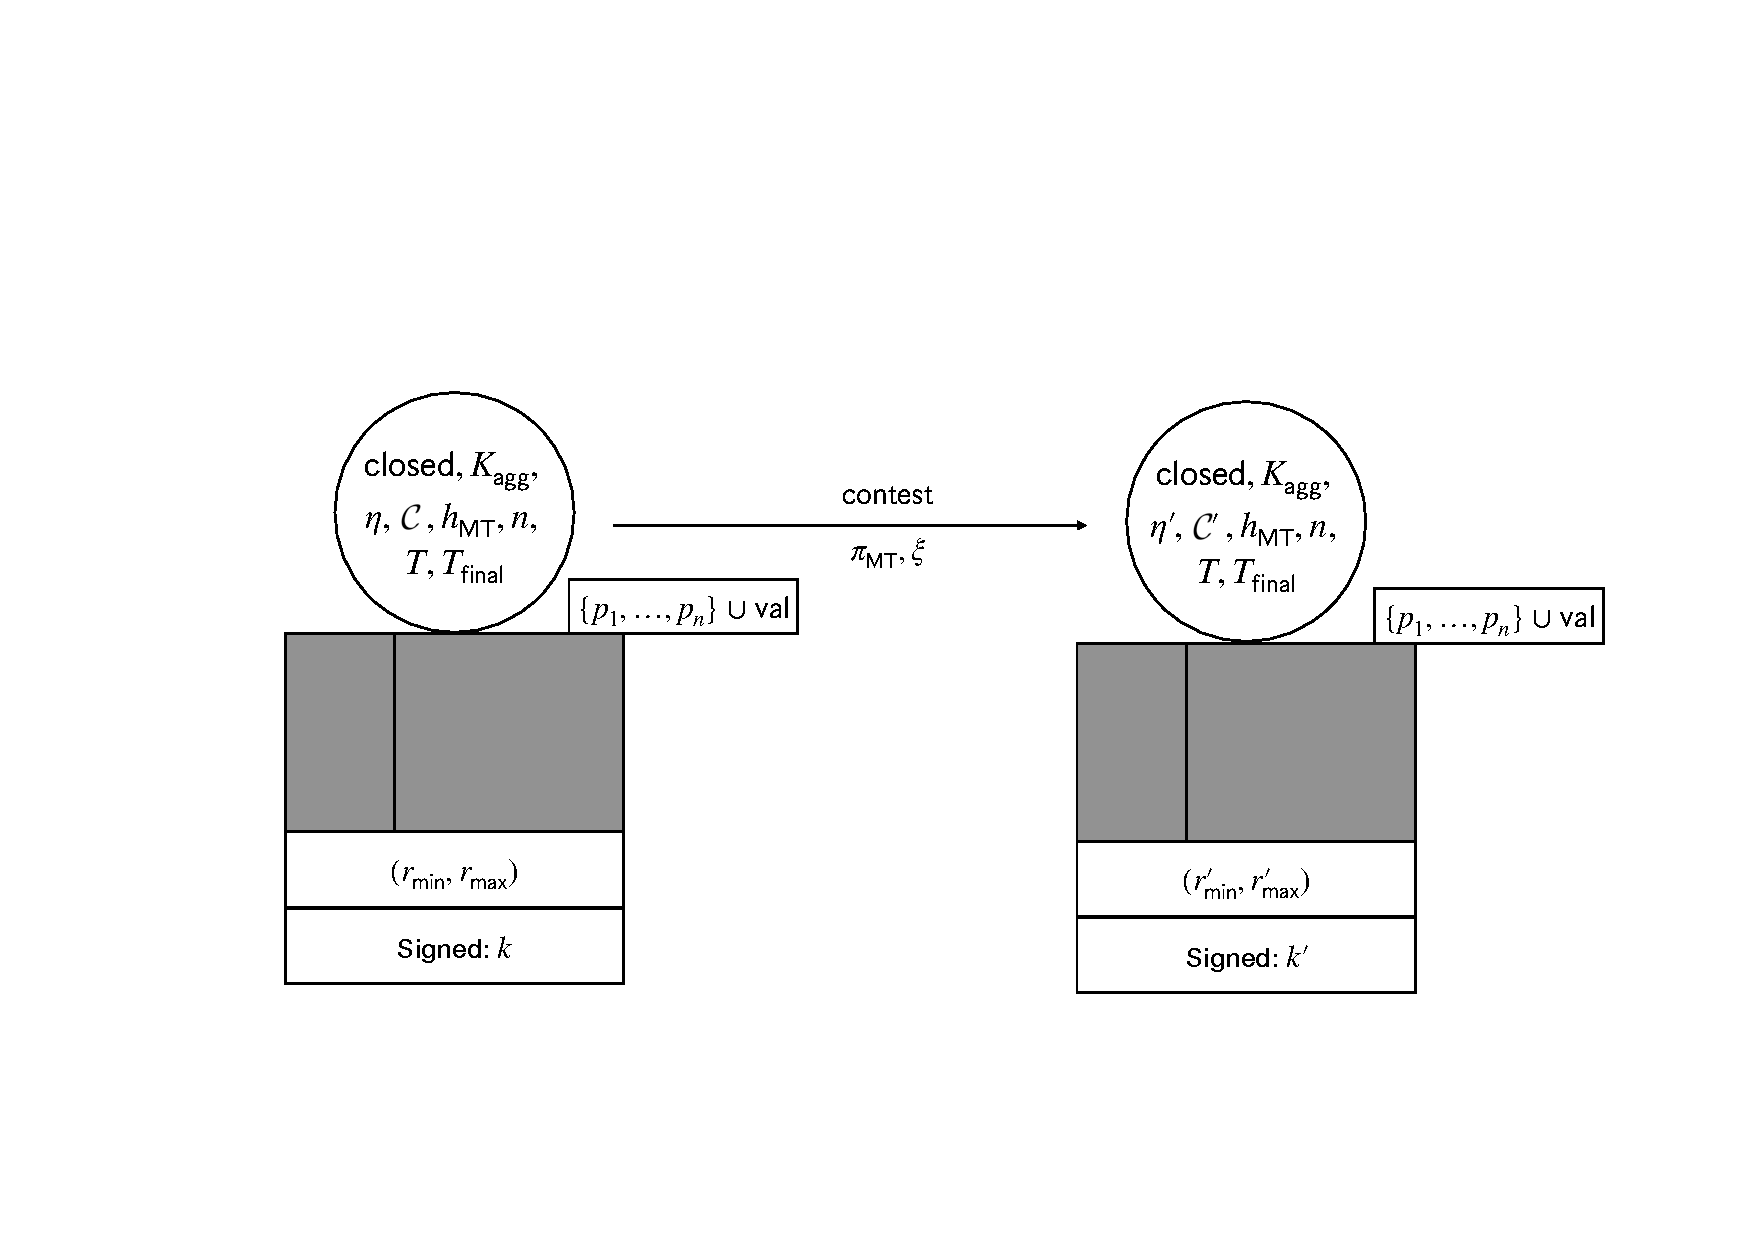
\includegraphics[width=\textwidth/2-2em,trim=280 120 160 260,
  %clip]{figures/SM_closed_closed.pdf}

  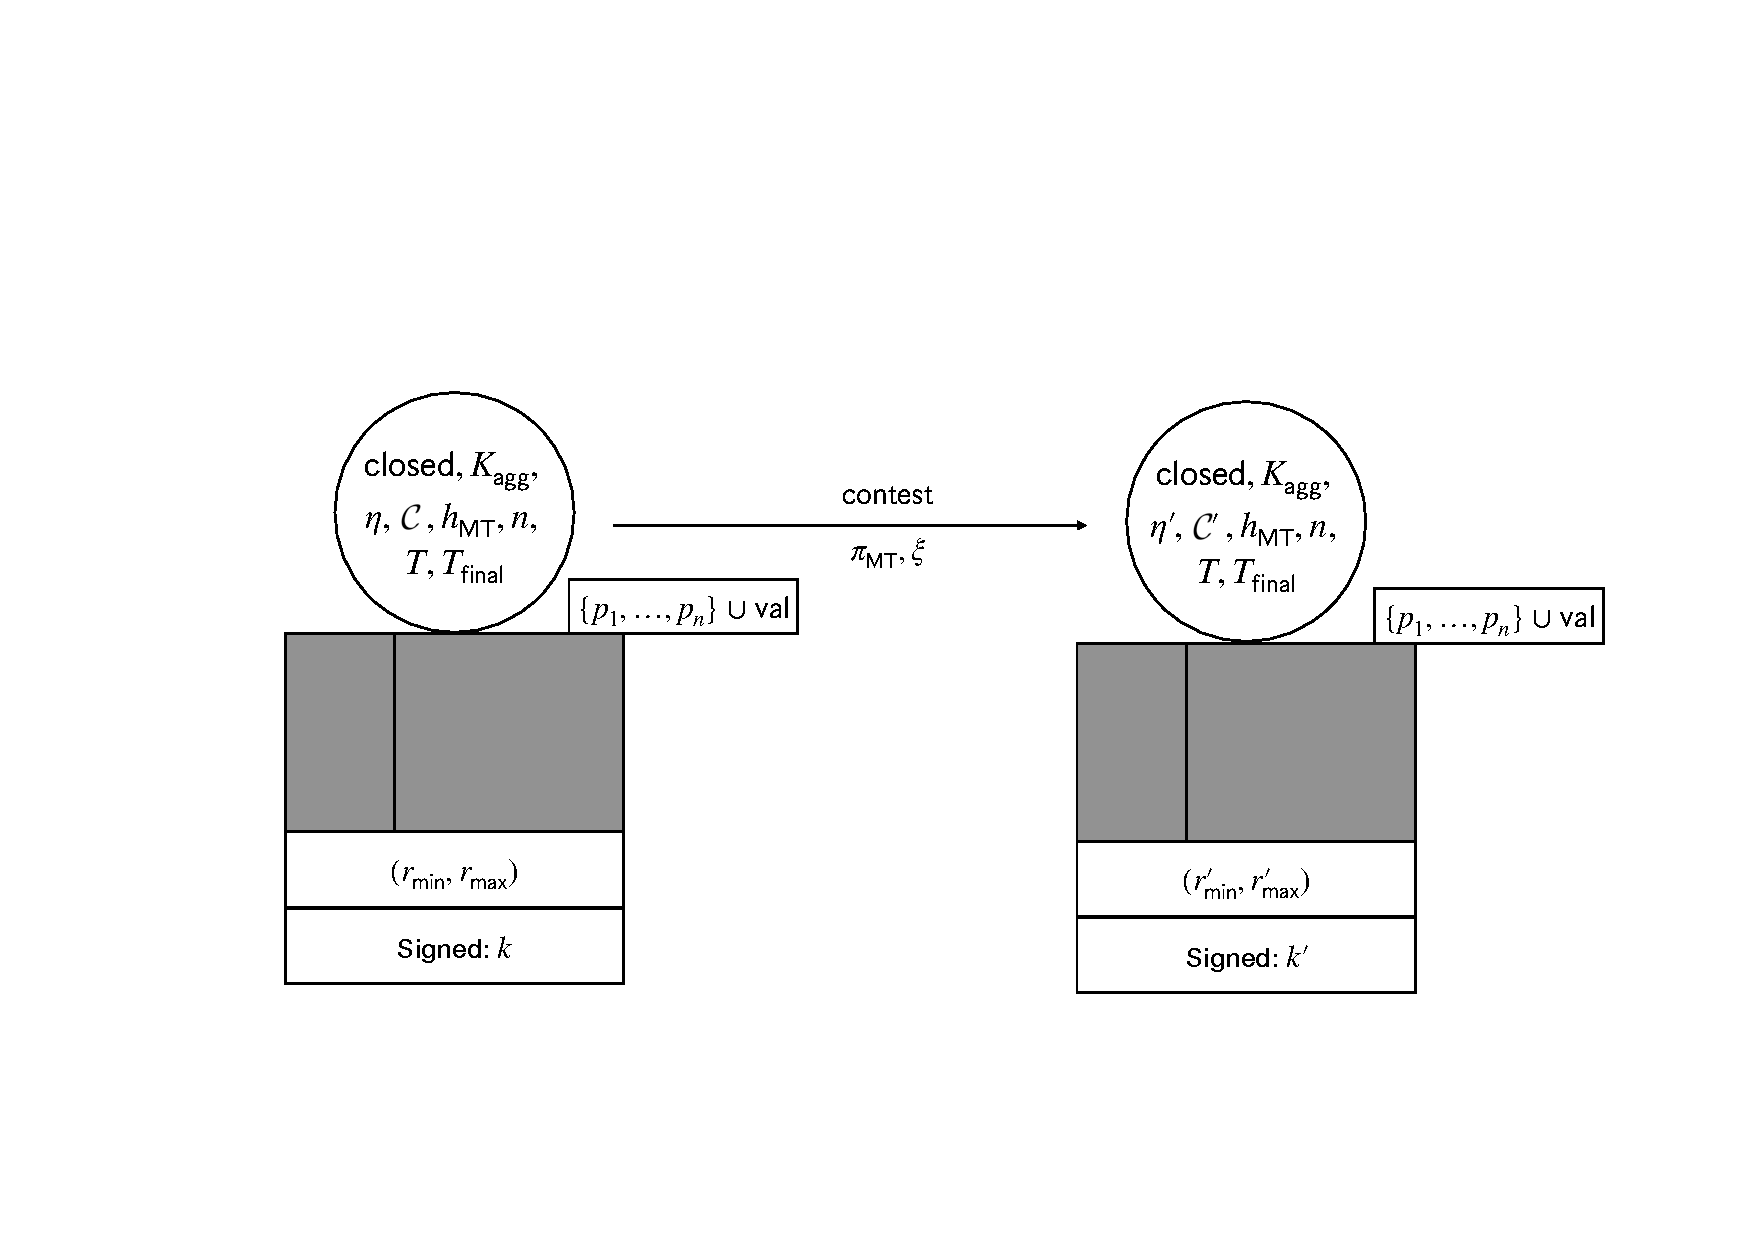
\includegraphics[width=\textwidth/2]{figures/SM_closed_closed.pdf}

  \caption{\mtxClose{}/\mtxContest{} transaction (left);
    \mtxContest{} transaction (right)}
  \label{fig:SM_closed_closed}

\end{figure}



%%% Local Variables:
%%% mode: latex
%%% TeX-master: "main"
%%% End:


The \mtxContest{} transaction (see
Fig.~\ref{fig:SM_closed_closed}) is posted by a party to prove the currently $\stClosed$ state is not the latest one. This causes the following transition in the CEM state machine (eg. change datum of output locked by $\nuHead$ script):
$$
   (\stClosed,\hpAK,\eta,\eta_0,\mathcal{C},\hppuv,\nop,\cPer,\Tfinal) \xrightarrow[\xi]{\mathsf{contest}} (\stClosed,\hpAK,\eta',\eta_0,\mathcal{C}', \hppuv,\nop,\cPer,\Tfinal'),
$$
with $\eta = (s, \hash(U))$ and $\eta' = (s', \hash(U')).$ \\

\noindent The $\nuHead$ validator additionally checks that:
\begin{menumerate}
  \item Value is preserved $\val' = \val$,
  \item Signer is one of the participants: $\txKeys = \{\mathsf{k'}\}$, $k' \in \hppuv$ and
    $
    \exists (\mathsf{cid} \rightarrow \mathsf{PT}_i \rightarrow 1) \in \val, \hash(\mathsf{k'}) = \mathsf{PT}_i,
    $
  \item The signer has not already contested $k' \not\in \mathcal{C},$  and it's added to the signers set: $\mathcal{C}' = \mathcal{C} \cup k',$
  \item $\xi$ is a valid multi-signature of $(\eta_0 || \eta')$ with respect to $\hpAK$, 
  \item $s' > s$, 
  \item Transaction is posted before deadline: $\txRmax \leq \Tfinal$,
  \item Contestation deadline is updated:
     $$
     \Tfinal' = 
        \left\{\begin{array}{ll}
             \Tfinal,     &  |\mathcal{C}'| = n, \\
             \Tfinal + T, &  \mathit{otherwise} \\
        \end{array}\right.,
     $$
  \item No minting or burning happens.
\end{menumerate}


\subsection{Fan-Out Transaction}  

\begin{figure}

  \centering

  % 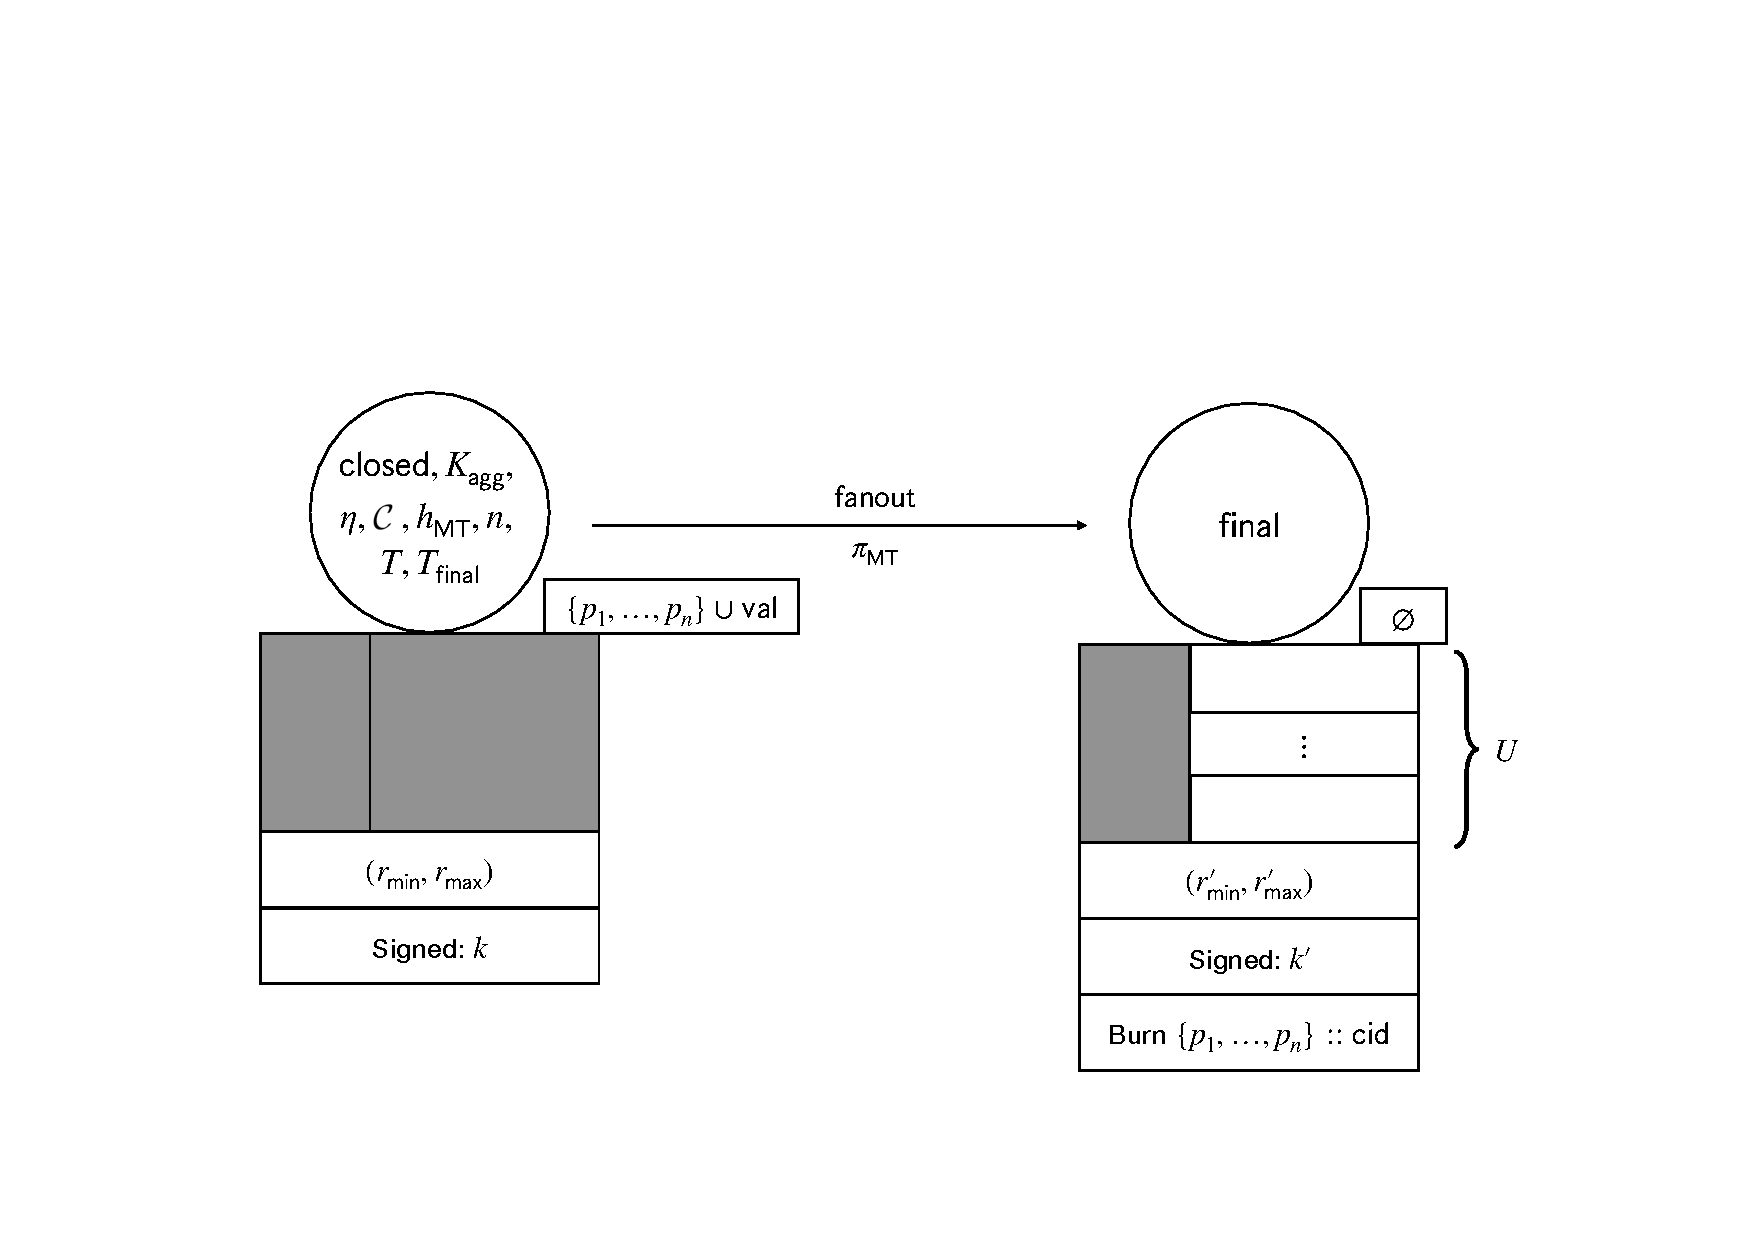
\includegraphics[width=\textwidth/2]{figures/SM_closed_final.pdf}

  % TODO: clean draw marked up version
  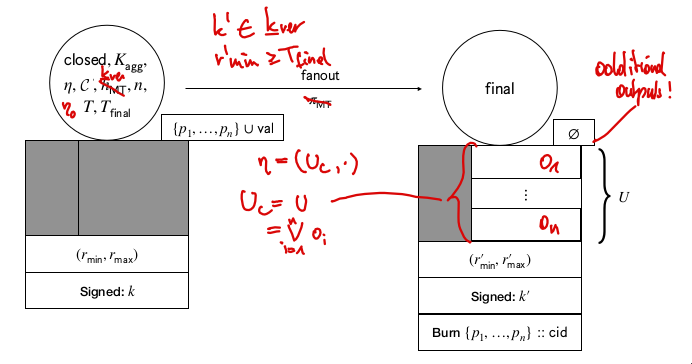
\includegraphics[width=\textwidth/2]{figures/SM_closed_final.png}

  \caption{\mtxClose{}/\mtxContest{} transaction (left);
    \mtxFanout{} transaction (right)}\label{fig:SM_closed_final}

\end{figure}

%%% Local Variables:
%%% mode: latex
%%% TeX-master: "main"
%%% End:


Once the contestation phase is over, a head
may be finalized by posting a \mtxFanout{} transaction, taking the SM
from $\stClosed$ to $\stFinal$.  

$$
   (\stClosed,\hpAK,\eta,\eta_0,\mathcal{C},\hppuv,\nop,\cPer,\Tfinal) \xrightarrow{\mathsf{fanout}} \stFinal,
$$
with $\eta = (s, H)$ and $\eta_0 = (0, H_0).$
The $\nuHead$ validator performs the following checks:
\begin{enumerate}
  \item Correct outputs are created: 
  $$
  \hash(\bigoplus_{i=1}^n \bytes(O[i])) = 
    \left\{
    \begin{array}{ll}
        H_0, & s = 0 \\
        H, &\mathit{otherwise}
    \end{array}
    \right.,
  $$
  \item All tokens are burnt: 
     $\mathsf{ST} \cup \{(\mathsf{cid} \rightarrow \mathsf{PT}_i \rightarrow -1) \mid i \in \{1\dots\nop\}\} \subseteq \mathsf{Mint},$
  \item Transaction is posted after contestation deadline $\txRmin > \Tfinal.$
\end{enumerate}

%%% Local Variables:
%%% mode: latex
%%% TeX-master: "main"
%%% End:
